\documentclass{article}

\usepackage[a4paper, bottom=0.5in, top=0.5in, left=0.5in, right=0.5in]{geometry}
\usepackage{wrapfig}
\usepackage{natbib}
\usepackage{url}
\usepackage{xcolor}
\usepackage{caption}
\usepackage{hyperref}
\hypersetup{
    colorlinks=true,    
    urlcolor=cyan,
}
\usepackage{bytefield}

\usepackage{amsfonts}
\usepackage{float}
\usepackage{enumitem}

\usepackage{minted}

\usepackage{xparse} % NewDocumentCommand, IfValueTF, IFBooleanTF
\usepackage{tikz-timing}[2014/10/29]
\NewDocumentCommand{\busref}{som}{\texttt{%
		#3%
		\IfValueTF{#2}{[#2]}{}%
		\IfBooleanTF{#1}{\#}{}%
}}


\newcommand{\bitFormat}[1]{\emph{\textbf{\textcolor{cyan}{#1}}}}

\newcommand{\regFormat}[1]{\textbf{\textcolor{magenta}{#1}}}

\newcommand{\pinFormat}[1]{\emph{\textcolor{red}{#1}}}


\usepackage{graphicx}
\graphicspath{ {./Resources/pics/} }



\title{ATmega328P Timer/Counter 1}
\author{Narendiran S}
\date{\today}

\begin{document}
\maketitle

\section{Features}
\begin{itemize}
    \item General purpose 16-bit PWM/Counter module.
    \item Two independent output compare units and One input capture unit
    \item Variable PWM.
    \item Four independent interrupt sources (TOV1, OCF0A, OCF1B and ICF1).
    \item Clear timer on compare match (auto reload)
\end{itemize}

\section{Block Diagram}
\begin{figure}[H]
    \begin{center}
        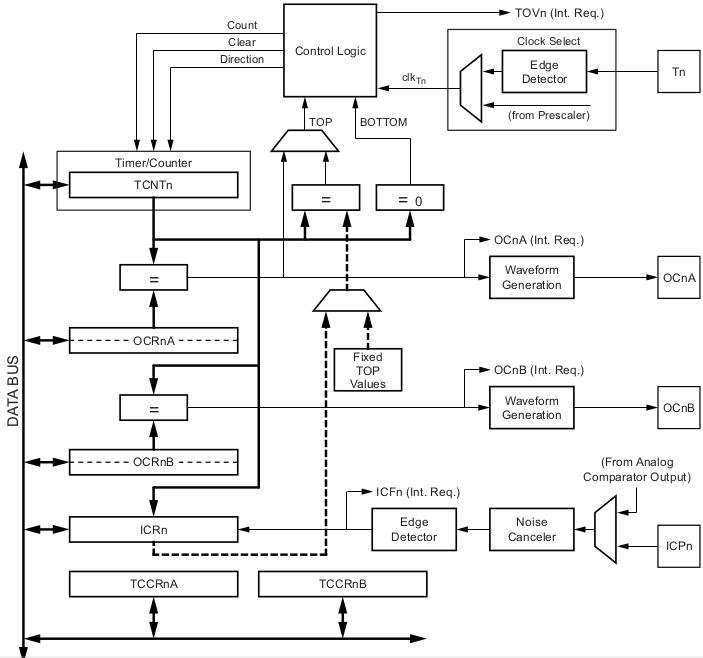
\includegraphics[height=0.6\textheight]{Timer1BlockDiagram.png}
    \end{center}
\end{figure}

\section{Terminologies and Registers}
\begin{minipage}{0.4\textwidth}
    \begin{tabular}{c|p{4.5cm}}
        \textbf{Parameter} & \textbf{Description}\\
        \hline
        BOTTOM & counter reaches 0x0000\\
        MAX & ounter reaches 0xFFFF\\
        TOP & counter reaches highest value (depends on mode of operation can be 0xFF, 0x1FF, 0x3FF, OCR1A, ICR1)
    \end{tabular}
\end{minipage}
\begin{minipage}{0.55\textwidth}
    \begin{tabular}{c|p{5.5cm}}
        \textbf{Register - 16 bit} & \textbf{Name}\\
        \hline
        \regFormat{TCN10} & Timer/Counter1count value\\
        \regFormat{TCCR1A} & Timer/Coutner1 Control Register A\\
        \regFormat{TCCR1B} & Timer/Coutner1 Control Register B\\
        \regFormat{OCBR1A} & Output compare register A\\
        \regFormat{OCBR1B} & Output compare register B\\
        \regFormat{TIFR1} & Timer Interrupt Flag Register\\
        \regFormat{TIMSK1} & Timer interrupt Mask Register\\
        \regFormat{ICR1} & Input Capture Register\\
    \end{tabular}
\end{minipage}

\textbf{Note: } 
\begin{itemize}
    \item The CNT1, OCR1A/B, and ICR1 are 16-bit registers that can be accessed by the CPU via the 8-bit data bus.
    \item \textbf{For 16-bit write, the high byte must be written before the low byte.}
    \item \textbf{For 16-bit read, the low byte must be read before the high byte.}
\end{itemize}
\section{Timer/Counter1 Units}

\subsection{Clock Source/Select Unit}
\begin{figure}[H]
    \begin{center}
        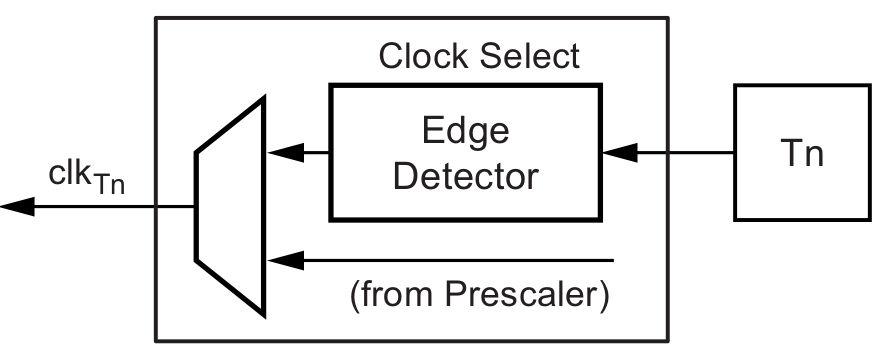
\includegraphics[width=0.5\textwidth]{Timer0ClockSelector.png}
    \end{center}
\end{figure}
\begin{itemize}
    \item The source for the Timer/Counter0 can be external or internal.
    \item External clock source is from \pinFormat{T1} pin.
    \item While Internal Clock source can be clocked via a prescalar.
    \item The output of this unit is the timer clock ($clk_{T1}$).
    \item It uses \bitFormat{CS1[2:0]} bits in \regFormat{TCCR1B} register to select the source.
\end{itemize}


\subsection{Counter Unit}
\begin{minipage}{0.5\textwidth}
    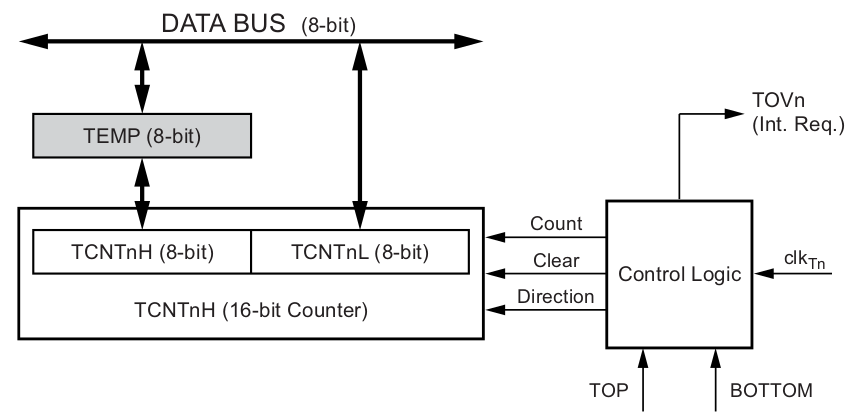
\includegraphics[width=1\textwidth]{Timer1CounterUnit.png}
\end{minipage}
\begin{minipage}{0.45\textwidth}
    \begin{tabular}{c|p{5.5cm}}
        \textbf{Signal} & \textbf{Description}\\
        \hline  
        count & Increment or decrement TCNT1 by 1\\
        direction & Select between increment or decrement\\
        clear & Clears TCNT1 to 0x0000\\
        $clk_{T1}$ & Timer/Coutner1 clock\\
        top & Signalize that TCNT1 has maximum value\\
        bottom & Signalize that TCNT1 has minimum value(0x0000)\\
    \end{tabular}
\end{minipage}
\begin{itemize}
    \item The main part of the 16-bit Timer/Counter is the programmable bi-directional counter.
    \item Counter high (TCNT1H) containing the upper eight bits of the counter, and counter low (TCNT1L) containing the lower eight bits.
    \item Depending the mode of operation the counter is cleared, incremented, or decremented at each timer clock ($clk_{T1}$).
    \item Counting sequence is determined by \bitFormat{WGM1[3:0]} bits of \regFormat{TCCR1A} -Timer/Counter1 Control register A and \regFormat{TCCR1B} - Timer/Counter1 Control register B.
    \item The Timer/Counter1 Overflow flag \bitFormat{(TOV1)} is set and can generate interrupt according to the mode.
\end{itemize}

\subsection{Input Capture Unit}
\begin{figure}[H]
    \centering
    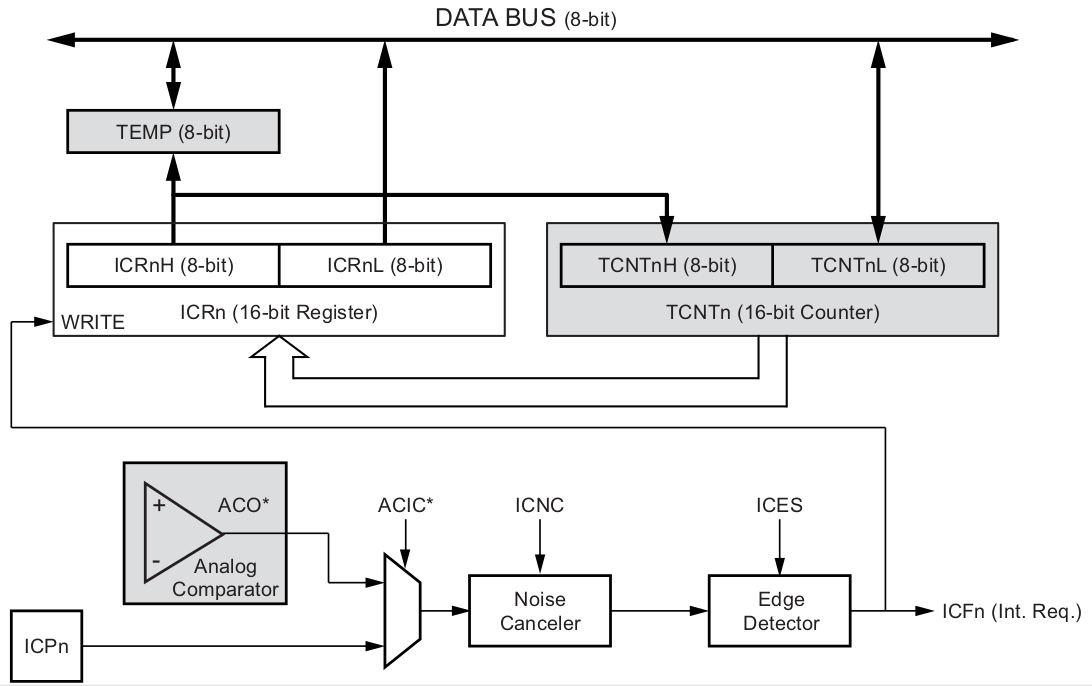
\includegraphics[width=0.75\textwidth]{Timer1InputCapture.png}
\end{figure}
\begin{itemize}
    \item Can capture external events and give them time-stamp indicating time of occurance.
    \item External signal can be from ICP1 pin or analog-comparator unit.
    \item Usage : calculate frequency, duty-cycle, log of the signal
    \item When a change of the logic level (an event) occurs on the input capture pin (\pinFormat{ICP1}), or on the analog comparator output (\pinFormat{ACO)}, and this change confirms to the setting of the edge detector, a capture will be triggered. 
    \item When a capture is triggered, the 16-bit value of the counter (\regFormat{TCNT1}) is written to the input capture register (\regFormat{ICR1}).
    \item The input capture flag (\bitFormat{ICF1}) is set at the same system clock as the \regFormat{TCNT1} value is copied into \regFormat{ICR1} register. 
    \item If enabled (\bitFormat{ICIE1} = 1), the input capture flag generates an input capture interrupt.
    \item \bitFormat{ICF1} flag is automatically cleared when the interrupt is executed and by writing on to i.
    \item An input capture can be triggered by software by controlling the port of the \pinFormat{ICP1} pin.
\end{itemize}

\subsection{Output Compare Unit}
\begin{figure}[H]
    \begin{center}
        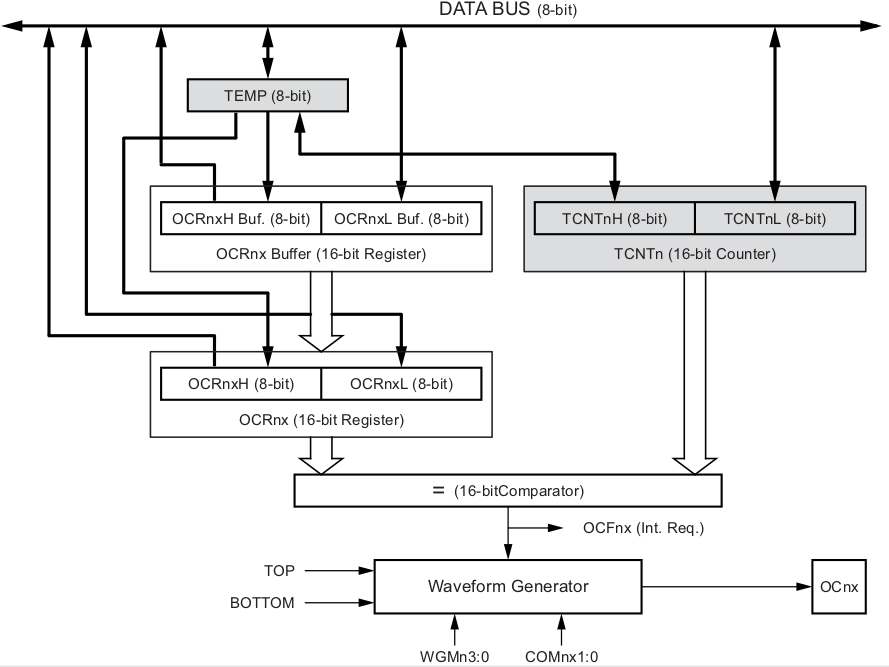
\includegraphics[width=0.6\textwidth]{Timer1OutputCompare.png}
    \end{center}
\end{figure}
\begin{itemize}
    \item 16-bit comparator continuously compares \regFormat{TCNT1} with both \regFormat{OCR1A} and \regFormat{OCR1B}.
    \item When \regFormat{TCNT1} equals \regFormat{OCR1A} or \regFormat{OCR1B}, the comparator signals a match which will set the output compare flag at the next timer clock cycle.
    \item If interrupts are enabled, then output compare interrupt is generated.
    \item The waveform generator uses the match signal to generate an output according to operating mode set by the \bitFormat{WGM1[3:0]} bits and compare output mode \bitFormat{COM0x[1:0]} bits.
\end{itemize}

\subsection{Compare Match Output Unit}
\begin{figure}[H]
    \begin{center}
        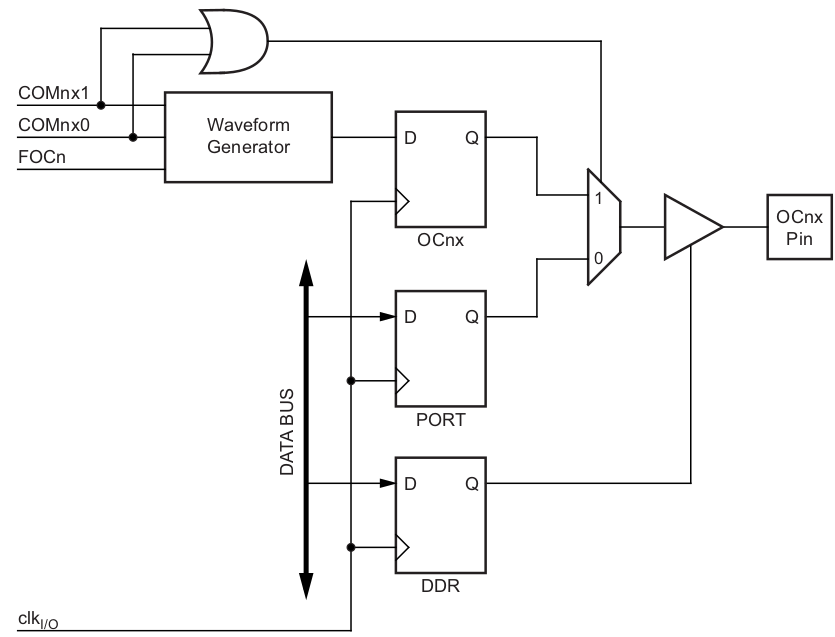
\includegraphics[height=0.3\textheight]{Timer1ComparteMatchOutput.png}
    \end{center}
\end{figure}
\begin{itemize}
    \item This unit is used for changing the state of \pinFormat{OC1A} and \pinFormat{OC1B} pins by configuring the \bitFormat{COM1x[1:0]} bits.
    \item But, general I/O port function is overriiden by DDR reigster.
\end{itemize}


\section{Modes of Operation}
\begin{itemize}
    \item The mode of operation can be defined by combination of waveform generation mode (\bitFormat{WGM1[3:0]}) and compare output mode(\bitFormat{COM1[1:0]}) bits.
    \item The waveform generation mode (\bitFormat{WGM1[3:0]}) bits affect the counting sequence.
    \item For non-PWM mode, \bitFormat{COM1[1:0]} bits control if the output should be set, cleared or toggled at a compare match.
    \item For PWM mode, \bitFormat{COM1[1:0]} bits control if the PWM generated should be inverted or non-inverted.
\end{itemize}



\subsection{Normal Mode - Non-PWM Mode}
\begin{itemize}
    \item WGM1[3:0] $-->$ 000.
    \item Counter counts up and no counter clear.
    \item Overruns TOP(0XFFFF) and restarts from BOTTOM(0X0000).
    \item \bitFormat{TOV1} Flag is only set when overrun.
    \item We have to clear \bitFormat{TOV1} flag inorder to have next running.
    \item But, if we use interrupt we don’t need to clear it as interrupt automatically clear the \bitFormat{TOV1} flag.
    \item The input capture unit can be used to capture events at \pinFormat{ICP1} pin or \pinFormat{ACO} pin.
    \item The timing can be seen below.
\end{itemize}

\begin{tikztimingtable}[
    timing/dslope=0.1,
    timing/.style={x=5ex,y=2ex},
    x=5ex,
    timing/rowdist=3ex,
    timing/name/.style={font=\sffamily\scriptsize}
    ]
    \busref{clk\_{T1}}  & 41{c}\\
    \busref{TCNT1} & u{} D{0x0000} D{0x0001};[dotted] 2D{};D{0xFFFE} D{0xFFFF}D{0x0000} D{0x0001};[dotted] 2D{};D{0xFFFE} D{0xFFFF}D{0x0000} D{0x0001};[dotted] 2D{};D{0xFFFE} D{0xFFFF}D{0x0000} D{0x0001}\\
    \busref{TOV1} & l 6{L} H 5{L} H 5{L} H 1{L}\\
\end{tikztimingtable}



\subsection{Clear Timer on Compare Match(CTC) Mode - Non-PWM Mode}
\begin{itemize}
    \item WGM1[3:0] $-->$ 0100 or 1100.
    \begin{itemize}
        \item Counter value clears when \regFormat{TCNT1} reaches \regFormat{OCR1A} if WGM1[3:0] is 0100.
        \item Counter value clears when \regFormat{TCNT1} reaches \regFormat{ICR1} if WGM1[3:0] is 1100.
    \end{itemize}
    \item Interrupt can be generated each time \regFormat{TCNT1} reaches \regFormat{OCR1A} register value by \bitFormat{OCF1A} flag.
    \item Interrupt can be generated each time \regFormat{TCNT1} reaches \regFormat{ICR1} register value by \bitFormat{ICF1} flag.
    \item When \bitFormat{COM1A[1:0]} == 01, the \pinFormat{OC1A} pin output can be set to toggle its match between \regFormat{TCNT1} and \regFormat{OCR1A} or \regFormat{ICR1} register to generate waveform.
    \item The frequency of the waveform its
    \begin{center}
        { \Large $f_{OC1A} = \frac{f_{clkT1}}{2 * N * (1 + OCR1A)}$ }
    \end{center}
    \item Here N is prescalar factor and can be (1, 8, 64, 256, or 1024).
\end{itemize}


\subsubsection{WGM1[3:0] == 0100}
\begin{tikztimingtable}[
    timing/dslope=0.1,
    timing/.style={x=5ex,y=2ex},
    x=5ex,
    timing/rowdist=3ex,
    timing/name/.style={font=\sffamily\scriptsize}
    ]
    \busref{clk\_{T1}}  & 28{1.5c}\\
    \busref{TCNT1} & 0.75U{} 1.5D{0x0000} 1.5D{0x0001};[dotted] 3D{};1.5D{OCR1A - 1} 1.5D{OCR1A}1.5D{0x0000} 1.5D{0x0001};[dotted] 3D{};1.5D{OCR1A - 1} 1.5D{OCR1A} 1.5D{0x0000} 0.75D{0x0001} \\
    \busref{OC1A} & 0.75L 9{L} 1.5H l 7{L} 1.5H l\\
\end{tikztimingtable}
\subsubsection{WGM1[3:0] == 1100}
\begin{tikztimingtable}[
    timing/dslope=0.1,
    timing/.style={x=5ex,y=2ex},
    x=5ex,
    timing/rowdist=3ex,
    timing/name/.style={font=\sffamily\scriptsize}
    ]
    \busref{clk\_{T1}}  & 28{1.5c}\\
    \busref{TCNT1} & 0.75U{} 1.5D{0x0000} 1.5D{0x0001};[dotted] 3D{};1.5D{ICR1 - 1} 1.5D{ICR1}1.5D{0x0000} 1.5D{0x0001};[dotted] 3D{};1.5D{ICR1 - 1} 1.5D{ICR1} 1.5D{0x0000} 0.75D{0x0001} \\
    \busref{OC1A} & 0.75L 9{L} 1.5H l 7{L} 1.5H l\\
\end{tikztimingtable}

\subsection{Fast PWM Mode}
\begin{itemize}
    \item WGM1[3:0] $-->$ 0101 or 0110 or 0111 or 1110 or 1111.
    \item Power Regulation, Rectification, DAC applications.
    \item Single slope operations causing high frequency PWM waveform.
    \item Counter starts from BOTTOM to TOP and then restarts from BOTTOM.
    \item TOP is defined by
    \begin{itemize}
        \item TOP == 0x00FF if WGM1[3:0] $-->$ 0101
        \item TOP == 0x01FF if WGM1[3:0] $-->$ 0110
        \item TOP == 0x03FF if WGM1[3:0] $-->$ 0111
        \item TOP ==   ICR1 if WGM1[3:0] $-->$ 1110
        \item TOP ==  OCR1A if WGM1[3:0] $-->$ 1111
    \end{itemize}
    \item  When \bitFormat{COM1A[1:0]} == 01, the \pinFormat{OC1A} pin output can be set to toggle its match between \regFormat{TCNT1} and TOP to generate waveform.
    \begin{itemize}
        \item The above is possible only when \bitFormat{WGM12} bit is set.
        \item And only on \pinFormat{OC1A} pin and not on \pinFormat{OC1B} pin.
    \end{itemize}
    \item In Inverting Compare Mode \bitFormat{COM1A[1:0]} == 10 , the \pinFormat{OC1A} or \pinFormat{OC1B} pins is made 1 on compare match between \regFormat{TCNT1} and TOP and made 0 on reaching BOTTOM.
    \item In Non-Inverting Compare Mode \bitFormat{COM1A[1:0]} == 11 , the \pinFormat{OC1A} or \pinFormat{OC1B} pins is made 0 on compare match between \regFormat{TCNT1} and TOP and 1 made  on reaching BOTTOM.
    \item The Timer/Counter overflow flag (\bitFormat{TOV1}) is set each time the counter reaches TOP.
    \item The PWM frequency is given by 
    \begin{center}
        { \Large $f_{OC1xPWM} = \frac{f_{clkT1}}{N * (1+ TOP)}$ }
    \end{center}
\end{itemize}

\subsubsection{WGM1[3:0] == 0101}
\begin{tikztimingtable}[
    timing/dslope=0.1,
    timing/.style={x=5ex,y=2ex},
    x=5ex,
    timing/rowdist=3ex,
    timing/name/.style={font=\sffamily\scriptsize}
    ]
    \busref{clk\_{T0}}  & 41{1c} c\\
    \busref{TCNT1} & 0.5U{} D{0x0000} 1D{0x0001};[dotted] 1.5D{};1D{0x00FE} 1D{0x00FF}1D{0x0000} 1D{0x0001};[dotted] 1D{};1D{0x00FE} 1D{0x00FF} 1D{0x0000} 1D{0x0001} [dotted] 1D{};1D{0x00FE} 1D{0x00FF} 1D{0x0000} 1D{0x0001};[dotted] 1D{};1D{0x00FE} 1D{0x00FF};\\
    \busref{TOV1} & 6{L} H 4{L} H 4{L} H 4{L} \\
\end{tikztimingtable}

\subsubsection{WGM1[3:0] == 0110}
\begin{tikztimingtable}[
    timing/dslope=0.1,
    timing/.style={x=5ex,y=2ex},
    x=5ex,
    timing/rowdist=3ex,
    timing/name/.style={font=\sffamily\scriptsize}
    ]
    \busref{clk\_{T0}}  & 41{1c} c\\
    \busref{TCNT1} & 0.5U{} D{0x0000} 1D{0x0001};[dotted] 1.5D{};1D{0x01FE} 1D{0x01FF}1D{0x0000} 1D{0x0001};[dotted] 1D{};1D{0x01FE} 1D{0x01FF} 1D{0x0000} 1D{0x0001} [dotted] 1D{};1D{0x01FE} 1D{0x01FF} 1D{0x0000} 1D{0x0001};[dotted] 1D{};1D{0x01FE} 1D{0x01FF};\\
    \busref{TOV1} & 6{L} H 4{L} H 4{L} H 4{L} \\
\end{tikztimingtable}
\subsubsection{WGM1[3:0] == 0111}
\begin{tikztimingtable}[
    timing/dslope=0.1,
    timing/.style={x=5ex,y=2ex},
    x=5ex,
    timing/rowdist=3ex,
    timing/name/.style={font=\sffamily\scriptsize}
    ]
    \busref{clk\_{T0}}  & 41{1c} c\\
    \busref{TCNT1} & 0.5U{} D{0x0000} 1D{0x0001};[dotted] 1.5D{};1D{0x03FE} 1D{0x03FF}1D{0x0000} 1D{0x0001};[dotted] 1D{};1D{0x03FE} 1D{0x03FF} 1D{0x0000} 1D{0x0001} [dotted] 1D{};1D{0x03FE} 1D{0x03FF} 1D{0x0000} 1D{0x0001};[dotted] 1D{};1D{0x03FE} 1D{0x03FF};\\
    \busref{TOV1} & 6{L} H 4{L} H 4{L} H 4{L} \\
\end{tikztimingtable}

\subsubsection{WGM1[3:0] == 1110}
\begin{tikztimingtable}[
    timing/dslope=0.1,
    timing/.style={x=5ex,y=2ex},
    x=5ex,
    timing/rowdist=3ex,
    timing/name/.style={font=\sffamily\scriptsize}
    ]
    \busref{clk\_{T0}}  & 41{1c} c\\
    \busref{TCNT1} & 0.5U{} D{0x0000} 1D{0x001};[dotted] 1.5D{};1D{\tiny ICR1 -1} 1D{\tiny ICR1}1D{0x0000} 1D{0x0001};[dotted] 1D{};1D{\tiny ICR1 -1} 1D{\tiny ICR1} 1D{0x0000} 1D{0x0001} [dotted] 1D{};1D{\tiny ICR1 -1} 1D{\tiny ICR1} 1D{0x0000} 1D{0x0001};[dotted] 1D{};1D{\tiny ICR1 -1} 1D{\tiny ICR1};\\
    \busref{TOV1} & 6{L} H 4{L} H 4{L} H 4{L} \\
\end{tikztimingtable}

\subsubsection{WGM1[3:0] == 1111}
\begin{tikztimingtable}[
    timing/dslope=0.1,
    timing/.style={x=5ex,y=2ex},
    x=5ex,
    timing/rowdist=3ex,
    timing/name/.style={font=\sffamily\scriptsize}
    ]
    \busref{clk\_{T0}}  & 41{1c} c\\
    \busref{TCNT1} & 0.5U{} D{0x0000} 1D{0x001};[dotted] 1.5D{};1D{\tiny OCR1A -1} 1D{\tiny OCR1A}1D{0x0000} 1D{0x0001};[dotted] 1D{};1D{\tiny OCR1A -1} 1D{\tiny OCR1A} 1D{0x0000} 1D{0x0001} [dotted] 1D{};1D{\tiny OCR1A -1} 1D{\tiny OCR1A} 1D{0x0000} 1D{0x0001};[dotted] 1D{};1D{\tiny OCR1A -1} 1D{\tiny OCR1A};\\
    \busref{TOV1} & 6{L} H 4{L} H 4{L} H 4{L} \\
\end{tikztimingtable}

\subsection{Phase Correct PWM Mode}
\begin{itemize}
    \item WGM1[3:0] $-->$ 0001 or 0010 or 0011 or 1010 or 1011.    
    \item High resolution phase correct PWM.
    \item Motor control due to symmetric features
    \item Dual slope operations causing ower frequency PWM waveform.
    \item Counter starts from BOTTOM to TOP and then from TOP to BOTTOM.
    \item TOP is defined by
    \begin{itemize}
        \item TOP == 0x00FF if WGM1[3:0] $-->$ 0001
        \item TOP == 0x01FF if WGM1[3:0] $-->$ 0010
        \item TOP == 0x03FF if WGM1[3:0] $-->$ 0011
        \item TOP ==   ICR1 if WGM1[3:0] $-->$ 1010
        \item TOP ==  OCR1A if WGM1[3:0] $-->$ 1011
    \end{itemize}
    \item  When \bitFormat{COM1A[1:0]} == 01, the \pinFormat{OC1A} pin output can be set to toggle its match between \regFormat{TCNT1} and TOP to generate waveform.
    \begin{itemize}
        \item The above is possible only when \bitFormat{WGM12} bit is set.
        \item And only on \pinFormat{OC1A} pin and not on \pinFormat{OC1B} pin.
    \end{itemize}
    \item In Inverting Compare Mode \bitFormat{COM1A[1:0]} == 10 , the \pinFormat{OC1A} or \pinFormat{OC1B} pins is made 1 on compare match between \regFormat{TCNT1} and TOP and made 0 on reaching BOTTOM.
    \item In Non-Inverting Compare Mode \bitFormat{COM1A[1:0]} == 11 , the \pinFormat{OC1A} or \pinFormat{OC1B} pins is made 0 on compare match between \regFormat{TCNT1} and TOP and 1 made  on reaching BOTTOM.
    \item The Timer/Counter overflow flag (\bitFormat{TOV1}) is set each time the counter reaches BOTTOM..
    \item The PWM frequency is given by 
    \begin{center}
        { \Large $f_{OC1xPWM} = \frac{f_{clkT1}}{2 * N * TOP}$ }
    \end{center}
\end{itemize}


\subsubsection{WGM1[3:0] == 0001}
\begin{tikztimingtable}[
    timing/dslope=0.1,
    timing/.style={x=5ex,y=2ex},
    x=5ex,
    timing/rowdist=3ex,
    timing/name/.style={font=\sffamily\scriptsize}
    ]
    \busref{clk\_{T1}}  & 41{1c} c\\
    \busref{TCNT1} & 0.5U{} D{0x0000} 1D{0x0001};[dotted] 1.5D{};1D{0x00FE} 1D{0x00FF}1D{0x0000} 1D{0x0001};[dotted] 1D{};1D{0x00FE} 1D{0x00FF} 1D{0x0000} 1D{0x0001} [dotted] 1D{};1D{0x00FE} 1D{0x00FF} 1D{0x0000} 1D{0x0001};[dotted] 1D{};1D{0x00FE} 1D{0x00FF};\\
    \busref{TOV1} & 6{L} H 4{L} H 4{L} H 4{L} \\
\end{tikztimingtable}


\subsubsection{WGM1[3:0] == 0010}
\begin{tikztimingtable}[
    timing/dslope=0.1,
    timing/.style={x=5ex,y=2ex},
    x=5ex,
    timing/rowdist=3ex,
    timing/name/.style={font=\sffamily\scriptsize}
    ]
    \busref{clk\_{T1}}  & 41{1c} c\\
    \busref{TCNT1} & 0.5U{} D{0x0000} 1D{0x0001};[dotted] 1.5D{};1D{0x01FE} 1D{0x01FF}1D{0x0000} 1D{0x0001};[dotted] 1D{};1D{0x01FE} 1D{0x01FF} 1D{0x0000} 1D{0x0001} [dotted] 1D{};1D{0x01FE} 1D{0x01FF} 1D{0x0000} 1D{0x0001};[dotted] 1D{};1D{0x01FE} 1D{0x01FF};\\
    \busref{TOV1} & 6{L} H 4{L} H 4{L} H 4{L} \\
\end{tikztimingtable}

\subsubsection{WGM1[3:0] == 0011}
\begin{tikztimingtable}[
    timing/dslope=0.1,
    timing/.style={x=5ex,y=2ex},
    x=5ex,
    timing/rowdist=3ex,
    timing/name/.style={font=\sffamily\scriptsize}
    ]
    \busref{clk\_{T1}}  & 41{1c} c\\
    \busref{TCNT1} & 0.5U{} D{0x0000} 1D{0x0001};[dotted] 1.5D{};1D{0x03FE} 1D{0x03FF}1D{0x0000} 1D{0x0001};[dotted] 1D{};1D{0x03FE} 1D{0x03FF} 1D{0x0000} 1D{0x0001} [dotted] 1D{};1D{0x03FE} 1D{0x03FF} 1D{0x0000} 1D{0x0001};[dotted] 1D{};1D{0x03FE} 1D{0x03FF};\\
    \busref{TOV1} & 6{L} H 4{L} H 4{L} H 4{L} \\
\end{tikztimingtable}

\subsubsection{WGM[2:0] == 101}
\begin{tikztimingtable}[
    timing/dslope=0.1,
    timing/.style={x=5ex,y=2ex},
    x=5ex,
    timing/rowdist=3ex,
    timing/name/.style={font=\sffamily\scriptsize}
    ]
    \busref{clk\_{T1}}  & 41{1c}\\
    \busref{TCNT1} & 0.5U{} D{0x0000} 1D{0x0001};[dotted] 1.5D{};1D{\tiny OCR1A - 1} 1D{\tiny OCR1A}1D{\tiny OCR01-1} 1D{\tiny OCR1A-2};[dotted] 1D{};1D{0x0001} 1D{0x0000} 1D{0x0001}[dotted] 1D{};1D{\tiny OCR1A-1} 1D{\tiny OCR1A} 1D{\tiny OCR1A-1} 1D{\tiny OCR1A-2};[dotted] 1D{};1D{0x0001} 1D{0x0000} 1d{0x0001};\\
    \busref{TOV1} & l H l 8{L} H 8{L} H l\\
\end{tikztimingtable}

\subsubsection{WGM[2:0] == 101}
\begin{tikztimingtable}[
    timing/dslope=0.1,
    timing/.style={x=5ex,y=2ex},
    x=5ex,
    timing/rowdist=3ex,
    timing/name/.style={font=\sffamily\scriptsize}
    ]
    \busref{clk\_{T1}}  & 41{1c}\\
    \busref{TCNT1} & 0.5U{} D{0x0000} 1D{0x0001};[dotted] 1.5D{};1D{\tiny ICR1- 1} 1D{\tiny ICR1}1D{\tiny ICR1-1} 1D{\tiny ICR1-2};[dotted] 1D{};1D{0x0001} 1D{0x0000} 1D{0x0001}[dotted] 1D{};1D{\tiny ICR1-1} 1D{\tiny ICR1} 1D{\tiny ICR1-1} 1D{\tiny ICR1-2};[dotted] 1D{};1D{0x0001} 1D{0x0000} 1d{0x0001};\\
    \busref{TOV1} & l H l 8{L} H 8{L} H l\\
\end{tikztimingtable}


\end{document}